\documentclass{beamer}

\usetheme{Montpellier}
\usecolortheme[named=brown]{structure}

\usepackage[utf8]{inputenc}
\usepackage[ngermanb]{babel}
\usepackage{url}
\usepackage{hyperref}

% font definitions, try \usepackage{ae} instead of the following
% three lines if you don't like this look
\usepackage{mathptmx}
\usepackage[scaled=.90]{helvet}
\usepackage{courier}

\usepackage[T1]{fontenc}

\usepackage{amsmath}
\usepackage{amssymb}
\usepackage{multicol}

\subject{Mini-Projekt: Minimax-Maschine}
\title{Mini-Projekt: Minimax-Maschine}
\subtitle{Projekt Technische Informatik WS 2011/12}
\author{Gerion Entrup\\ Martin Matthaei\\ Sergej Wildemann\\ Sven Karsten Greiner\\ \\ (Gruppe 4)}
\date{\today}

\AtBeginSection[]
{
\begin{frame}<beamer>
\frametitle{Inhalt}
\tableofcontents[currentsection]
\end{frame}
}

% If you wish to uncover everything in a step-wise fashion, uncomment
% the following command:

%\beamerdefaultoverlayspecification{<+->}

\begin{document}



\begin{frame}
\titlepage
\end{frame}



\begin{frame}
\frametitle{Inhalt}
{
    % Nur Chapter und Section ins Inhaltsverzeichnis
    \setcounter{tocdepth}{2}
    \tableofcontents %[pausesections]
}
\end{frame}



\section{Einführung}

\subsection{Aufgabe}



\begin{frame}{Aufbau der Daten}

\begin{itemize}[<+->]
    \item im Hauptspeicher unterschiedliche Datenpakete
    \item jedes Paket enthält Kopf von 80 Bits und einen Datenteil mit variabler Länge
    \item Paket fängt mit Muster \texttt{1110} an
    \item im Kopfes ist die Kanalnummer in zwei nacheinander folgenden Bytes ab Bit 32 vertretet
    \item zu einem Kanal können mehrere Pakete mit eindeutiger Kanalnummer gehören
\end{itemize}

\end{frame}



\begin{frame}{Beispiel}

\begin{center}
    \begin{tabular}{|c|c|c|c|c|}
        \multicolumn{1}{c}{0-3} & \multicolumn{1}{c}{} & \multicolumn{1}{c}{32-47} & \multicolumn{1}{c}{48-79} & \multicolumn{1}{c}{} \\
        \hline
        1110 & xxx & Kanalnummer & xxx & \hspace{1cm} Datenteil \hspace{1cm} \\
        \hline
    \end{tabular}
\end{center}

\begin{center}
    \begin{tabular}{|c|c|c|c|c|c|c|c|c|}
        \hline
        H_0 & \hspace{.3cm} D_0 \hspace*{.3cm} & H_1 & D_1 & H_2 & \hspace{1cm} D_2 \hspace*{1cm} & ...... & H_n & D_n \\
        \hline
    \end{tabular}
\end{center}

\end{frame}



\begin{frame}[label=aufgabe]{Aufgabe}

\begin{itemize}
    \item Algorithmus für Minimax"=Maschine entwickeln\pause, welcher
\end{itemize}

\begin{itemize}
    \item Speichertabelle mit Kanalnummer und Datenlänge (in Bits) aller zugehörigen Pakete erstellt
    \item Tabelle an beliebiger Stelle im Hauptspeicher (außerhalb des Paketfeldbereiches) speichert
\end{itemize}

\pause

\begin{itemize}
    \item Länge des Paketfeldes als Parameter
    \item ACCU beinhaltet Startspeicheradresse
\end{itemize}

\end{frame}



\begin{frame}{Beispiel}

\begin{center}
    \tiny
    \begin{tabular}{|c|c|c|c|c|c|c|c|c|c|c|c|c|c|c|}
        \multicolumn{5}{c|}{1. Paket} & \multicolumn{5}{c|}{2. Paket} & \multicolumn{5}{c}{3. Paket}\\ \hline
        1110 & x & $243_{10}$ & x & 1001 & 1110 & x & $243_{10}$ & x & 10110 & 1110 & x & $3727_{10}$ & x & 1001 \\ \hline
    \end{tabular}
\end{center}

\begin{center}
    \footnotesize
    \begin{tabular}{|r|r|l|}
        \hline
        Kanalnr. & Anzahl \\
        \hline
        \hline
        243 & 9 \\
        \hline
        3727 & 4 \\
        \hline
    \end{tabular}
\end{center}

\end{frame}



\subsection{Minimax"=Maschine}

\subsubsection{Allgemeiner Aufbau}



\begin{frame}{Wie ist die Minimaxmaschine aufgebaut?}

\begin{figure}
    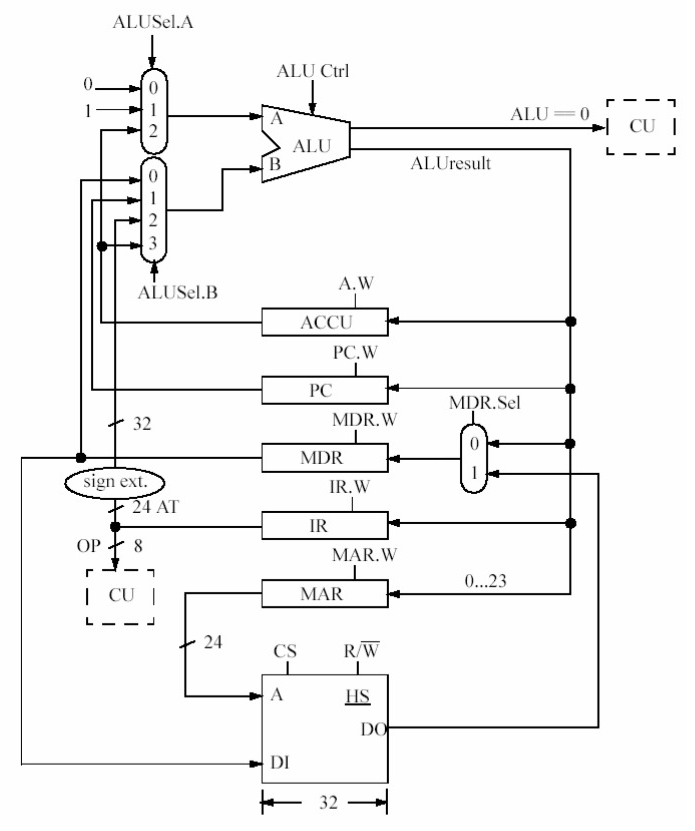
\includegraphics[width=0.4\textwidth]{res/minimax.png} 
    \caption{Schematische Darstellung der Minimax"=Maschine}
\end{figure}

\end{frame}



\begin{frame}{Basiskonfiguration}

\begin{description}
    \item[ACCU] \emph{Accumulator}, Zwischenspeicher
    \item[PC] \emph{Program Counter}, Zähler für Programmablauf
    \item[MDR] \emph{Memory Data Register}, Daten von/für Hauptspeicher
    \item[IR] \emph{Instruction Register}, enthält Opcode (8 Bit) mit Adressteil (24 Bit)
    \item[MAR] \emph{Memory Address Register}, enthält die Speicheradresse für HS
\end{description}

\end{frame}



\begin{frame}{Basiskonfiguration}

\begin{columns}[l]
    \column{.45\textwidth}
    \begin{block}{Multiplexer an ALU}
        \textbf{A:} 0, 1, ACCU\\
        \textbf{B:} MDR, PC, AT, ACCU
    \end{block}

    \column{.55\textwidth}
    \pause
    \begin{block}{ALU"=Operationen}
        \begin{description}
            \item[ADD] $ALUresult \gets A + B$
            \item[SUB.B] $ALUresult \gets -A + B$
            \item[TRANS.A] $ALUresult \gets A$
            \item[TRANS.B] $ALUresult \gets B$
        \end{description}
    \end{block}
\end{columns}

\end{frame}



\begin{frame}{Basiskonfiguration}

\begin{itemize}
    \item Hauptspeicher wird mit 24 Bit adressiert
    \item liefert Daten mit 32 Bit
\end{itemize}

\pause

\begin{itemize}
    \item Wenn ALU"=Operation mit Ergebnis \texttt{NULL}, dann Flag \texttt{ALU==0}
\end{itemize}

\end{frame}

\begin{frame}{Programm und Steuertabelle}
\begin{itemize}
    \item Auf der Maschine wird ein Programm ausgeführt,
    \item dass Befehle benutzt die in der Steuertabelle als Mikroprogramm stehen.
    \item korrekter Programmablauf durch IFETCH geregelt
\end{itemize}
\end{frame}

\subsubsection{Simulator}



\begin{frame}{Simulator}
\begin{itemize}
    \item Minimax-Maschine nicht in Hardware vorhanden
    \item stattdessen Simulator
    \item in Java geschrieben
    \item seit 8 Jahren nicht verbessert
\end{itemize}
\end{frame}



\section{Lösung}

\subsection{Lösungsansatz}



% Wir wollen uns nochmal die Aufgabe ins Gedächtnis holen, aha, wollen wir das bei einer präsentation wo alle das kennen? kp, kann man vllt. auch weglassen
%\againframe{aufgabe}



\begin{frame}{Lösungsansatz}
\begin{itemize}
    \item Ergebnistabelle im Speicher direkt hinter Paketen
    \item Kanalnr. nicht gespeichert, sondern in der Adresse codiert
    \item Mit zwei Puffern die Speicherzellen durchgehen, um die bitweise Verschiebung zu realisieren
    \item Unwichtige Teile des Paketheaders überspringen
\end{itemize}
\end{frame}



\subsection{Algorithmus als Flussdiagramm}



\begin{frame}{Flussdiagramm}

\begin{figure}
    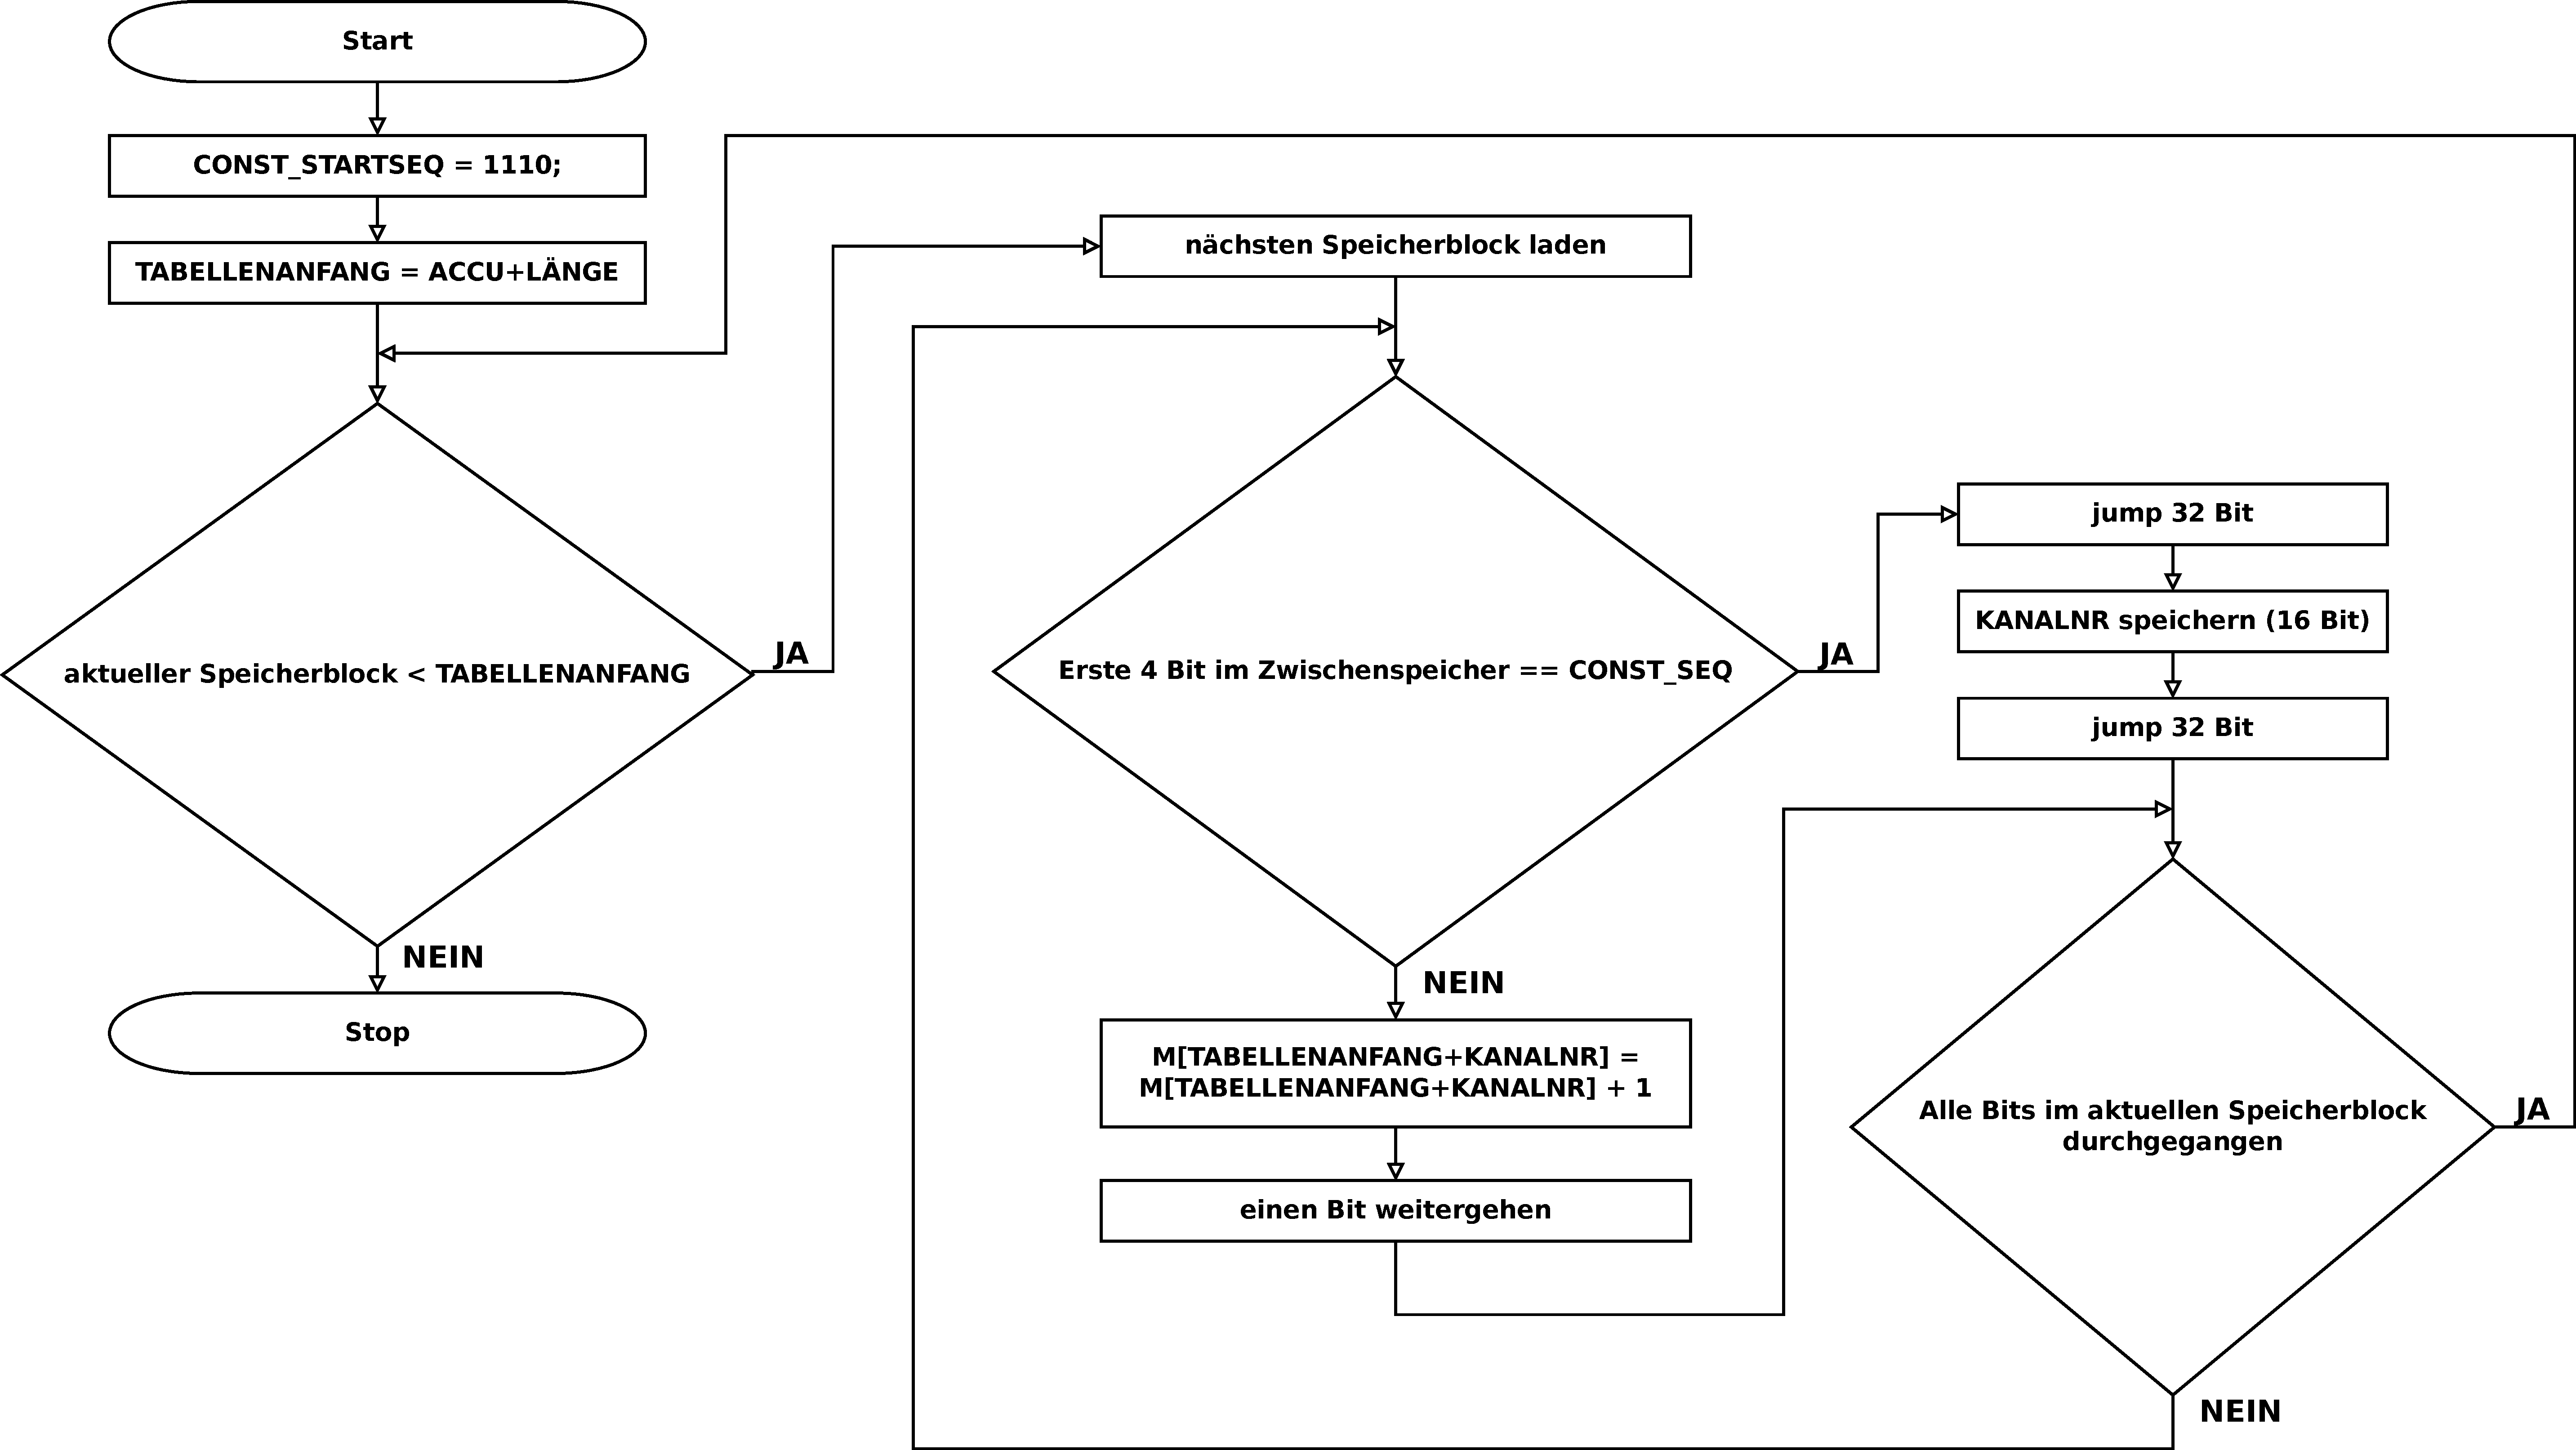
\includegraphics[width=\textwidth]{res/algorithmus.pdf}
\end{figure}

\end{frame}



\subsection{Übertragung von Flussdiagramm in konkreten Code}



\subsubsection{Erweiterungen}



\begin{frame}{Benötigte Erweiterungen}

\begin{block}{ALU"=Operationen:}
    \begin{center}
        \begin{tabular}{lc}
            Operation & Code \\
            \hline
            ADD       & 000 \\
            SUB.B     & 001 \\
            TRANS.A   & 010 \\
            TRANS.B   & 011 \\
            MUL       & 100 \\
            SR.B      & 101 \\
            AND       & 110 \\
        \end{tabular}
    \end{center}
\end{block}

\end{frame}



\begin{frame}{Benötigte Erweiterungen}
\begin{multicols}{2}
    \begin{block}{ALUSel.A:}
        \begin{tabular}{lcc}
            Quelle               & Code & Eingang \\
            \hline
            ACCU                 & 0000 &  0 \\
            0                    & 0001 &  1 \\
            1                    & 0010 &  2 \\
            (32)_{10}            & 0011 &  3 \\
            (2^{16})_{10}        & 0100 &  4 \\
            (2^{28})_{10}        & 0101 &  5 \\
            (2^{31})_{10}        & 0110 &  6 \\
            FILLED               & 0111 &  7 \\
            PC                   & 1000 &  8 \\
            KANALNR              & 1001 &  9 \\
            (2^4)_{10}           & 1010 & 10 \\
            (2)_{10}             & 1011 & 11 \\
        \end{tabular}
    \end{block}

    \columnbreak

    \begin{block}{ALUSel.B:}
        \begin{tabular}{lcc}
            Quelle        & Code & Eingang \\
            \hline
            ACCU          & 0000 &  0 \\
            MDR           & 0001 &  1 \\
            AT(signext)   & 0010 &  2 \\
            TABELLENANF   & 0011 &  3 \\
            BUFFER\_ONE   & 0100 &  4 \\
            BUFFER\_TWO   & 0101 &  5 \\
            FILLEDTMP     & 0110 &  6 \\
            FILLED        & 0111 &  7 \\
            PC            & 1000 &  8 \\
            (14)_{10}     & 1001 &  9 \\
        \end{tabular}
    \end{block}
\end{multicols}

\end{frame}



\subsubsection{Erkennung des Headers}



\begin{frame}[fragile]{Erkennung des Headers}

{\footnotesize\begin{verbatim}
ACCU <- 0xf
ACCU <- BUFFER_ONE && ACCU
STARTSEQ - ACCU == 0
    0,GOTO DATENTEIL
    1,GOTO HEADER
\end{verbatim}}
\begin{tabular}{ll}
DATENTEIL: & Bits werden gezählt\\
HEADER: & Kanalnr. speichern, den Rest überspringen
\end{tabular}

\end{frame}



\subsubsection{Shift}



\begin{frame}[fragile]{Shift}

{\footnotesize\begin{verbatim}
BUFFER_ONE <- shiftr BUFFER_ONE
ACCU <- BUFFER_TWO && 0x00000001
ACCU <- ACCU * 2^31
BUFFER_ONE <- BUFFER_ONE + ACCU
BUFFER_TWO <- shiftr BUFFER_TWO
\end{verbatim}}
\begin{tabular}{ll}
BUFFER\_ONE:& Bitgenau geshifteter Speicherinhalt\\
BUFFER\_TWO:& Speicher wird dort hereingeladen
\end{tabular}
\end{frame}



\subsubsection{Jump 32}



\begin{frame}[fragile]{Jump von 32 Bits}

{\footnotesize\begin{tabular}{|l|l|}
    \multicolumn{2}{l}{Ist-Zustand:}\\
    \hline
    Speicher   & \texttt{ccccccccccccbbbbbbbbbbbbbbbbbbbb}\\
    \hline
    \texttt{BUFFER\_ONE} & \texttt{egalegalegalegalegalegalegalegal}\\
    \hline
    \texttt{BUFFER\_TWO} & \texttt{00000000000000000000aaaaaaaaaaaa}\\
    \hline
    \multicolumn{2}{l}{}\\
    \multicolumn{2}{l}{Soll-Zustand:}\\
    \hline
    Speicher   & \texttt{ccccccccccccbbbbbbbbbbbbbbbbbbbb}\\
    \hline
    \texttt{BUFFER\_ONE} & \texttt{bbbbbbbbbbbbbbbbbbbbaaaaaaaaaaaa}\\
    \hline
    \texttt{BUFFER\_TWO} & \texttt{00000000000000000000cccccccccccc}\\
    \hline
\end{tabular}\\
\begin{verbatim}
BUFFER_ONE <- Speicher
BUFFER_ONE <- shiftl BUFFER_ONE (x-mal)
BUFFER_ONE <- BUFFER_ONE && BUFFER_TWO
BUFFER_TWO <- Speicher
BUFFER_TWO <- shiftr BUFFER_TWO ((32-x)-mal)
\end{verbatim}}

\end{frame}
%TODO muss der Algorithmus hier noch in RT-Notation hin? Ich würde ihn weglassen, nur grobes vorgehen erklären



\subsubsection{Kanalnr. speichern und Tabelle erstellen}



\begin{frame}[fragile]{Kanalnr. speichern und Tabelle erstellen}
\begin{block}{Kanalnr. speichern:}
{\footnotesize\begin{verbatim}
ACCU <- 2^16
ACCU <- ACCU - 1
KANALNR <- BUFFER_ONE && ACCU
\end{verbatim}}
\end{block}
\begin{block}{Tabelle erstellen:}
{\footnotesize\begin{verbatim}
MAR <- TABELLENANFANG + KANALNR
MDR <- M[MAR]
...
MDR <- MDR + 1
...
M[MAR] <- MDR
\end{verbatim}}
\end{block}
\end{frame}



\subsection{Praktische Vorführung}



\begin{frame}{Praktische Vorführung}

\begin{figure}
    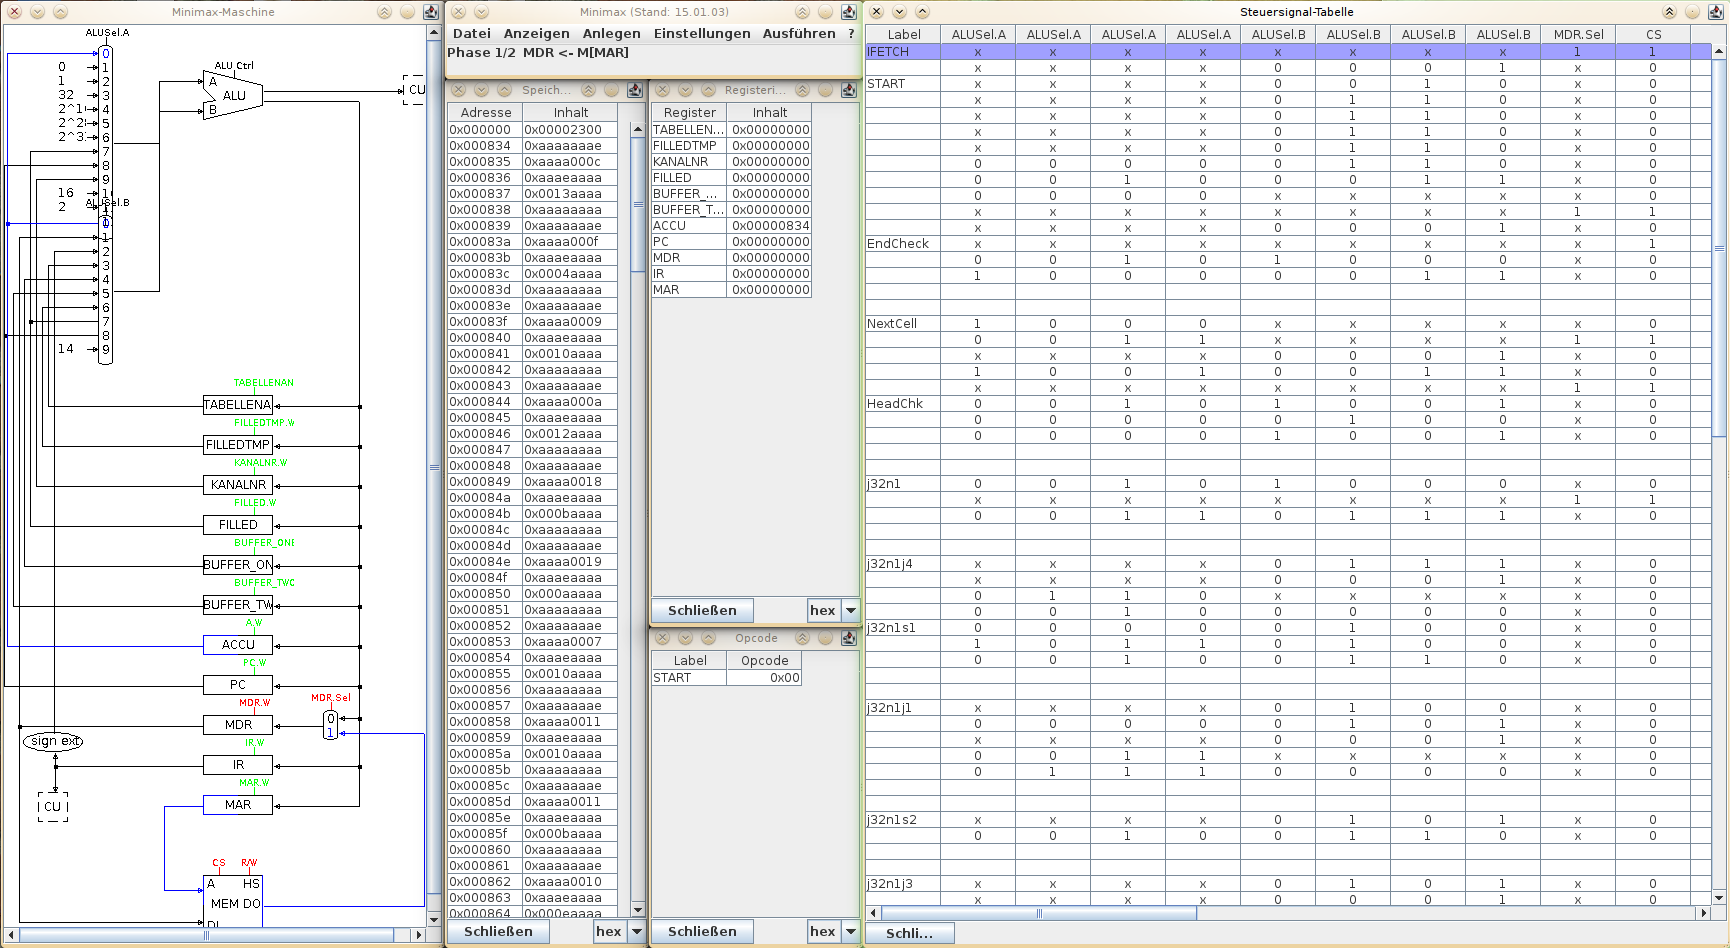
\includegraphics[width=\textwidth]{res/simulator.png}
\end{figure}

\end{frame}



\section{Ergebnis}



\subsection{Benchmark}



\begin{frame}{Werte}

{\footnotesize\begin{align*}
    reg      &= 6 \\
    se       &= 0 \\
    const    &= 7 \\ \\
    alu\_add &= MUL + AND + SR.B \\
             &= 16 + 6 + 5 = 27 \\ \\
    alu\_use &= 4 \cdot MUL + 6 \cdot AND + 14 \cdot SR.B \\
             &= 4 \cdot 16 + 6 \cdot 6 + 14 \cdot 5 = 170
\end{align*}}

\end{frame}



\begin{frame}{Laufzeit}

{\footnotesize\begin{align*}
    t_{bewertet} &= t_{bench} \cdot (1 + 0.1 \cdot reg + 0.15 \cdot se + 0.015 \cdot alu\_add + 0.05 \cdot const) \\
                 &= t_{bench} \cdot (1 + 0.1 \cdot 6 + 0.15 \cdot 0 + 0.015 \cdot 27 + 0.05 \cdot 7) \\
                 &= t_{bench} \cdot 2.355
\end{align*}}

\begin{center}
    \begin{tabular}{|l|l|r|}
        \hline
        Speicherabbild & Minimaxtakte & \multicolumn{1}{l|}{$t_{bewertet}$} \\
        \hline
        \hline
        1 & 24\,935 & 58\,721.925 \\
        \hline
        2 & 58\,423 & 137\,586.165 \\
        \hline
        3 & 67\,975 & 160\,081.125 \\
        \hline
    \end{tabular}
\end{center}

\end{frame}



\begin{frame}{Länge}

{\footnotesize\begin{align*}
    n_{bewertet} &= n_{Algorithmus} + 5 \cdot reg + 10 \cdot se + 3 \cdot alu\_use + 5 \cdot const \\
                 &= 118 + 5 \cdot 6 + 10 \cdot 0 + 3 \cdot 170 + 5 \cdot 7 \\
                 &= 118 + 575 \\
                 &= 693
\end{align*}}

\end{frame}



\begin{frame}{Ergebnistabellen}

\begin{multicols}{3}
    Benchmark 1:
    
    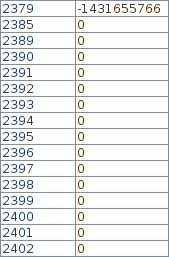
\includegraphics[width=0.25\textwidth]{res/bench1_result.png}
    \vfill
    \columnbreak
    
    Benchmark 2:
    
    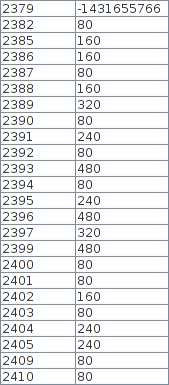
\includegraphics[width=0.25\textwidth]{res/bench2_result.png}
    \vfill
    \columnbreak
    
    Benchmark 3:
    
    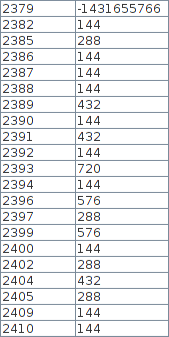
\includegraphics[width=0.25\textwidth]{res/bench3_result.png}
\end{multicols}

\end{frame}



\subsection{Bewertung} %TODO vllt mit Dokumentation mehr abgleichen?



\begin{frame}{Abschließende Bewertung}
\begin{itemize}
    \item Durch anfängliche Falschannahme bezüglich mehr Möglichkeiten des Simulators eventuell ineffizienten Algorithmus gewählt
    \item Optimierung unter Beibehaltung des Algorithmus
    \item Zufriedenstellendes Ergebnis für den Zeitaufwand
\end{itemize}
\end{frame}



%\section*{Quellen}

%\begin{frame}
%\frametitle{Quellen}

%\begin{itemize}
%  \item 
%\end{itemize}

%\end{frame}



\end{document}
